\section{Software Process Model}

The development of the AI-Driven Lab Exam Monitoring and Management System follows the Agile process model. Agile is particularly suitable for this project because the system contains several interdependent modules, requires continuous refinement of workflows, and must respond to user feedback related to usability, security, and academic practicality. In projects involving dashboards, access roles, examination rules, event logging, and post-exam reporting, it is difficult to finalize every detail correctly at the very beginning. Agile provides a controlled but iterative way to build the system in increments, validate assumptions early, and refine the product across repeated feedback cycles.

\subsection{Process Model Introduction}

Agile is an iterative and incremental development model in which software evolves through repeated short cycles called sprints. Each sprint focuses on a manageable subset of work and produces a meaningful improvement in the system. Rather than postponing user feedback until the final stage, Agile encourages continuous interaction between planning, implementation, review, and refinement. This makes it highly appropriate for academic systems where stakeholders often understand their needs more clearly after seeing early prototypes and working workflows.

In the context of the proposed system, Agile supports a practical balance between technical implementation and institutional feedback. An early sprint can validate whether the role-based dashboard structure is clear, while a later sprint can refine monitoring logic, face verification flow, or reporting outputs based on observed weaknesses. Such iterative evolution helps reduce the risk of investing too much effort in features that are technically complete but operationally unsuitable. It also helps the project remain realistic within semester constraints while still demonstrating meaningful progress \cite{pmc_cbt} \cite{mit_cbt}.

\begin{figure}[H]
\centering
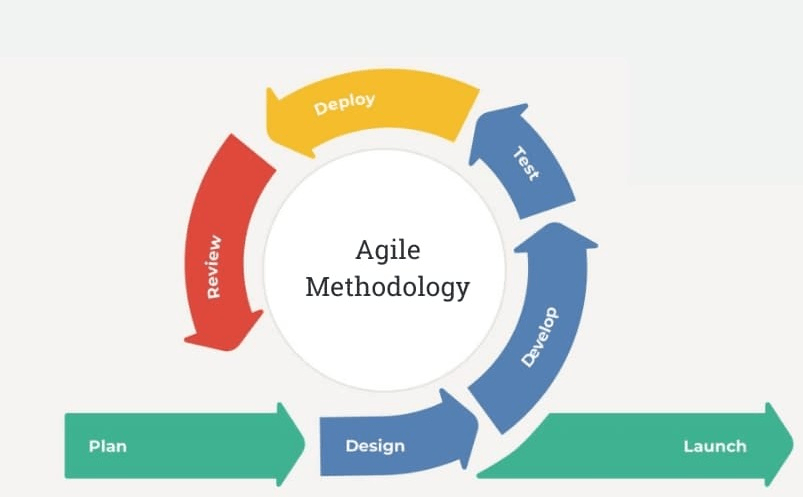
\includegraphics[width=0.97\linewidth]{Figures/agile_workflow_detailed.png}
\caption{Detailed Agile Workflow with Sprint Feedback and Review Loops}
\label{fig:agileworkflowdetailed}
\end{figure}

\subsection{Justification of Proposing the Process Model}

Agile is chosen over a rigid sequential model because the proposed system is not a single-purpose utility; it is a multi-role academic platform whose usefulness depends heavily on workflow suitability. A strictly linear process would assume that scheduling logic, monitoring interface needs, alert behavior, evidence presentation, and reporting expectations can all be finalized with certainty before implementation begins. In reality, these design decisions benefit from iterative refinement. A dashboard that appears clear on paper may prove cluttered in a simulated invigilation scenario. A submission flow that seems simple in design may become confusing when aligned with real timing rules. Agile offers a way to respond to such issues before they become deeply embedded in the system.

Agile is also appropriate because the FYP itself develops under academic review conditions. Supervisor input, testing observations, and prototype demonstrations all contribute to the maturity of the final result. Instead of viewing change as a disruption, Agile treats controlled change as a normal and productive part of development. This aligns well with a student project in which requirements become sharper through research, modeling, and demonstration. Furthermore, the modular nature of the proposed system means that high-priority features such as login, scheduling, monitoring, and evidence logging can be developed first, while secondary enhancements can be refined later without destabilizing the project.

\subsection{Steps of Process Model}

The Agile process model for this project is organized into eight sprints. Each sprint spans four weeks, which is treated as an approximately thirty-day working cycle for planning, implementation, review, and refinement. The twelve project modules are distributed across these eight sprints so that each increment produces a meaningful and reviewable outcome.

\textbf{Sprint 1 (Weeks 1--4):} Requirement Analysis and System Planning. This sprint establishes the project backlog and defines the architecture baseline. Activities include stakeholder discussion, use-case identification, product backlog preparation, initial workflow sketches, and approval of the project scope.

\textbf{Sprint 2 (Weeks 5--8):} Core Access Control and Authentication. This sprint focuses on secure access to the platform. The modules delivered are Authentication and Device Binding (Module 1) and User and Role Management (Module 7). Activities include designing JWT login endpoints, HWID extraction libraries, user registration interfaces, role permissions, and dashboard routing for administrators, teachers, and students.

\textbf{Sprint 3 (Weeks 9--12):} Exam Configuration and Administration. This sprint addresses academic setup before the live exam. The modules delivered are Exam Creation and Configuration (Module 8) and Eligibility and Access Control (Module 9). Activities include setting up exam templates, configuring allowed applications lists, coding test case definitions, exam seat assignment logic, and manual teacher overrides.

\textbf{Sprint 4 (Weeks 13--16):} Student Desktop Client Environment. This sprint develops the secure workspace for test-taking. The modules delivered are Pre-Exam System Verification and Mock Test (Module 2), Exam Dashboard (Module 3), and Secure Exam Environment Module (Module 4). Activities include student WPF lockdown client dashboard, fullscreen locked mode (disabling Alt+Tab, Task Manager), and client readiness verification checks.

\textbf{Sprint 5 (Weeks 17--20):} Live Telemetry and Proctoring. This sprint strengthens live session invigilation. The modules delivered are Live Monitoring Client Service (Module 5) and Live Proctoring Dashboard (Module 10). Activities include background focus tracking and process list logging, heartbeat synchronization, and real-time focus timeline grid view on the React teacher dashboard.

\textbf{Sprint 6 (Weeks 21--24):} Submission and AI Evaluation. This sprint handles post-exam grading. The modules delivered are Exam Submission and Backup (Module 6) and AI-Assisted Evaluation Module (Module 11). Activities include answer auto-save, local encrypted backups, automated execution against test cases, AI theory evaluation, and intra-class plagiarism comparison matrix.

\textbf{Sprint 7 (Weeks 25--28):} Reporting, Analytics, and Auditing. This sprint handles the system auditing and reports. The modules delivered are Logs, Analytics and Audit Trail System (Module 12). Activities include log management, database audit logs, system performance stats, and QuestPDF generation for downloadable analytical exam reports.

\textbf{Sprint 8 (Weeks 29--32):} Integration, Testing, and Final Refinement. This sprint consolidates all previously completed work into one stable prototype. Activities include module integration, usability improvement, bug fixing, end-to-end testing, sprint review closure, documentation completion, and preparation of final academic deliverables for demonstration and report submission.
